%\documentclass{beamer}
\documentclass[handout]{beamer}
\usetheme{Marburg}
\useoutertheme{infolines}
\newcommand{\answers}{1}

\usepackage{amsmath}
\usepackage{caption}
\usepackage{color}
\usepackage{enumerate}
\usepackage{listings}
\usepackage{hyperref}
\usepackage{mathrsfs}
\usepackage{setspace}
\usepackage{tikz}
\usepackage{tkz-graph}
\usepackage{url}

\providecommand{\all}{\ \forall \ }
\providecommand{\bs}{\backslash}
\providecommand{\e}{\varepsilon}
\providecommand{\E}{\ \exists \ }
\providecommand{\lm}[2]{\lim_{#1 \rightarrow #2}}
\providecommand{\m}[1]{\mathbb{#1}}
\providecommand{\mc}[1]{\mathcal{#1}}
\providecommand{\nv}{{}^{-1}}
\providecommand{\ov}[1]{\overline{#1}}
\providecommand{\p}{\newpage}
\providecommand{\q}{$\quad$ \newline}
\providecommand{\rt}{\rightarrow}
\providecommand{\Rt}{\Rightarrow}
\providecommand{\vc}[1]{\boldsymbol{#1}}
\providecommand{\wh}[1]{\widehat{#1}}

\hypersetup{colorlinks,linkcolor=,urlcolor=blue}
\numberwithin{equation}{section}

\definecolor{dkgreen}{rgb}{0,0.6,0}
\definecolor{gray}{rgb}{0.5,0.5,0.5}
\definecolor{mauve}{rgb}{0.58,0,0.82}

\lstset{ 
  language=C,                % the language of the code
  basicstyle= \footnotesize,           % the size of the fonts that are used for the code
  numbers=left,
  numberfirstline=true,
  numbersep=5pt,                  % how far the line-numbers are from the code
  backgroundcolor=\color{white},      % choose the background color. You must add \usepackage{color}
  showspaces=false,               % show spaces adding particular underscores
  showstringspaces=false,         % underline spaces within strings
  showtabs=false,                 % show tabs within strings adding particular underscores
  frame=lrb,                   % adds a frame around the code
  rulecolor=\color{black},        % if not set, the frame-color may be changed on line-breaks within not-black text 
  tabsize=2,                      % sets default tabsize to 2 spaces
  captionpos=t,                   % sets the caption-position 
  breaklines=true,                % sets automatic line breaking
  breakatwhitespace=false,        % sets if automatic breaks should only happen at whitespace
  %title=\lstname,                   % show the filename of files included with \lstinputlisting;
  keywordstyle=\color{blue},          % keyword style
  commentstyle=\color{gray},       % comment style
  stringstyle=\color{dkgreen},         % string literal style
  escapeinside={\%*}{*)},            % if you want to add LaTeX within your code
  morekeywords={*, ...},               % if you want to add more keywords to the set
  xleftmargin=0.053in, % left horizontal offset of caption box
  xrightmargin=-.03in % right horizontal offset of caption box
}

\DeclareCaptionFont{white}{\color{white}}
\DeclareCaptionFormat{listing}{\parbox{\textwidth}{\colorbox{gray}{\parbox{\textwidth}{#1#2#3}}}}
\captionsetup[lstlisting]{format = listing, labelfont = white, textfont = white}
 %For caption-free listings, comment out the 3 lines above
 \lstset{frame = single}

\title{The heterosis problem: a comparison of Eric's method with {\tt edgeR}, {\tt baySeq}, and {\tt ShrinkBayes}}
\author{Will Landau, Eric Mittman}
\date{\today}
\institute{Iowa State University}

\begin{document}

\begin{frame}
\titlepage
\end{frame}

 \AtBeginSection[]
{
   \begin{frame}
       \frametitle{Outline}
       \tableofcontents[currentsection]
   \end{frame}
}

\section{The problem}

\begin{frame}
\frametitle{Mock heterosis data}
\begin{center}
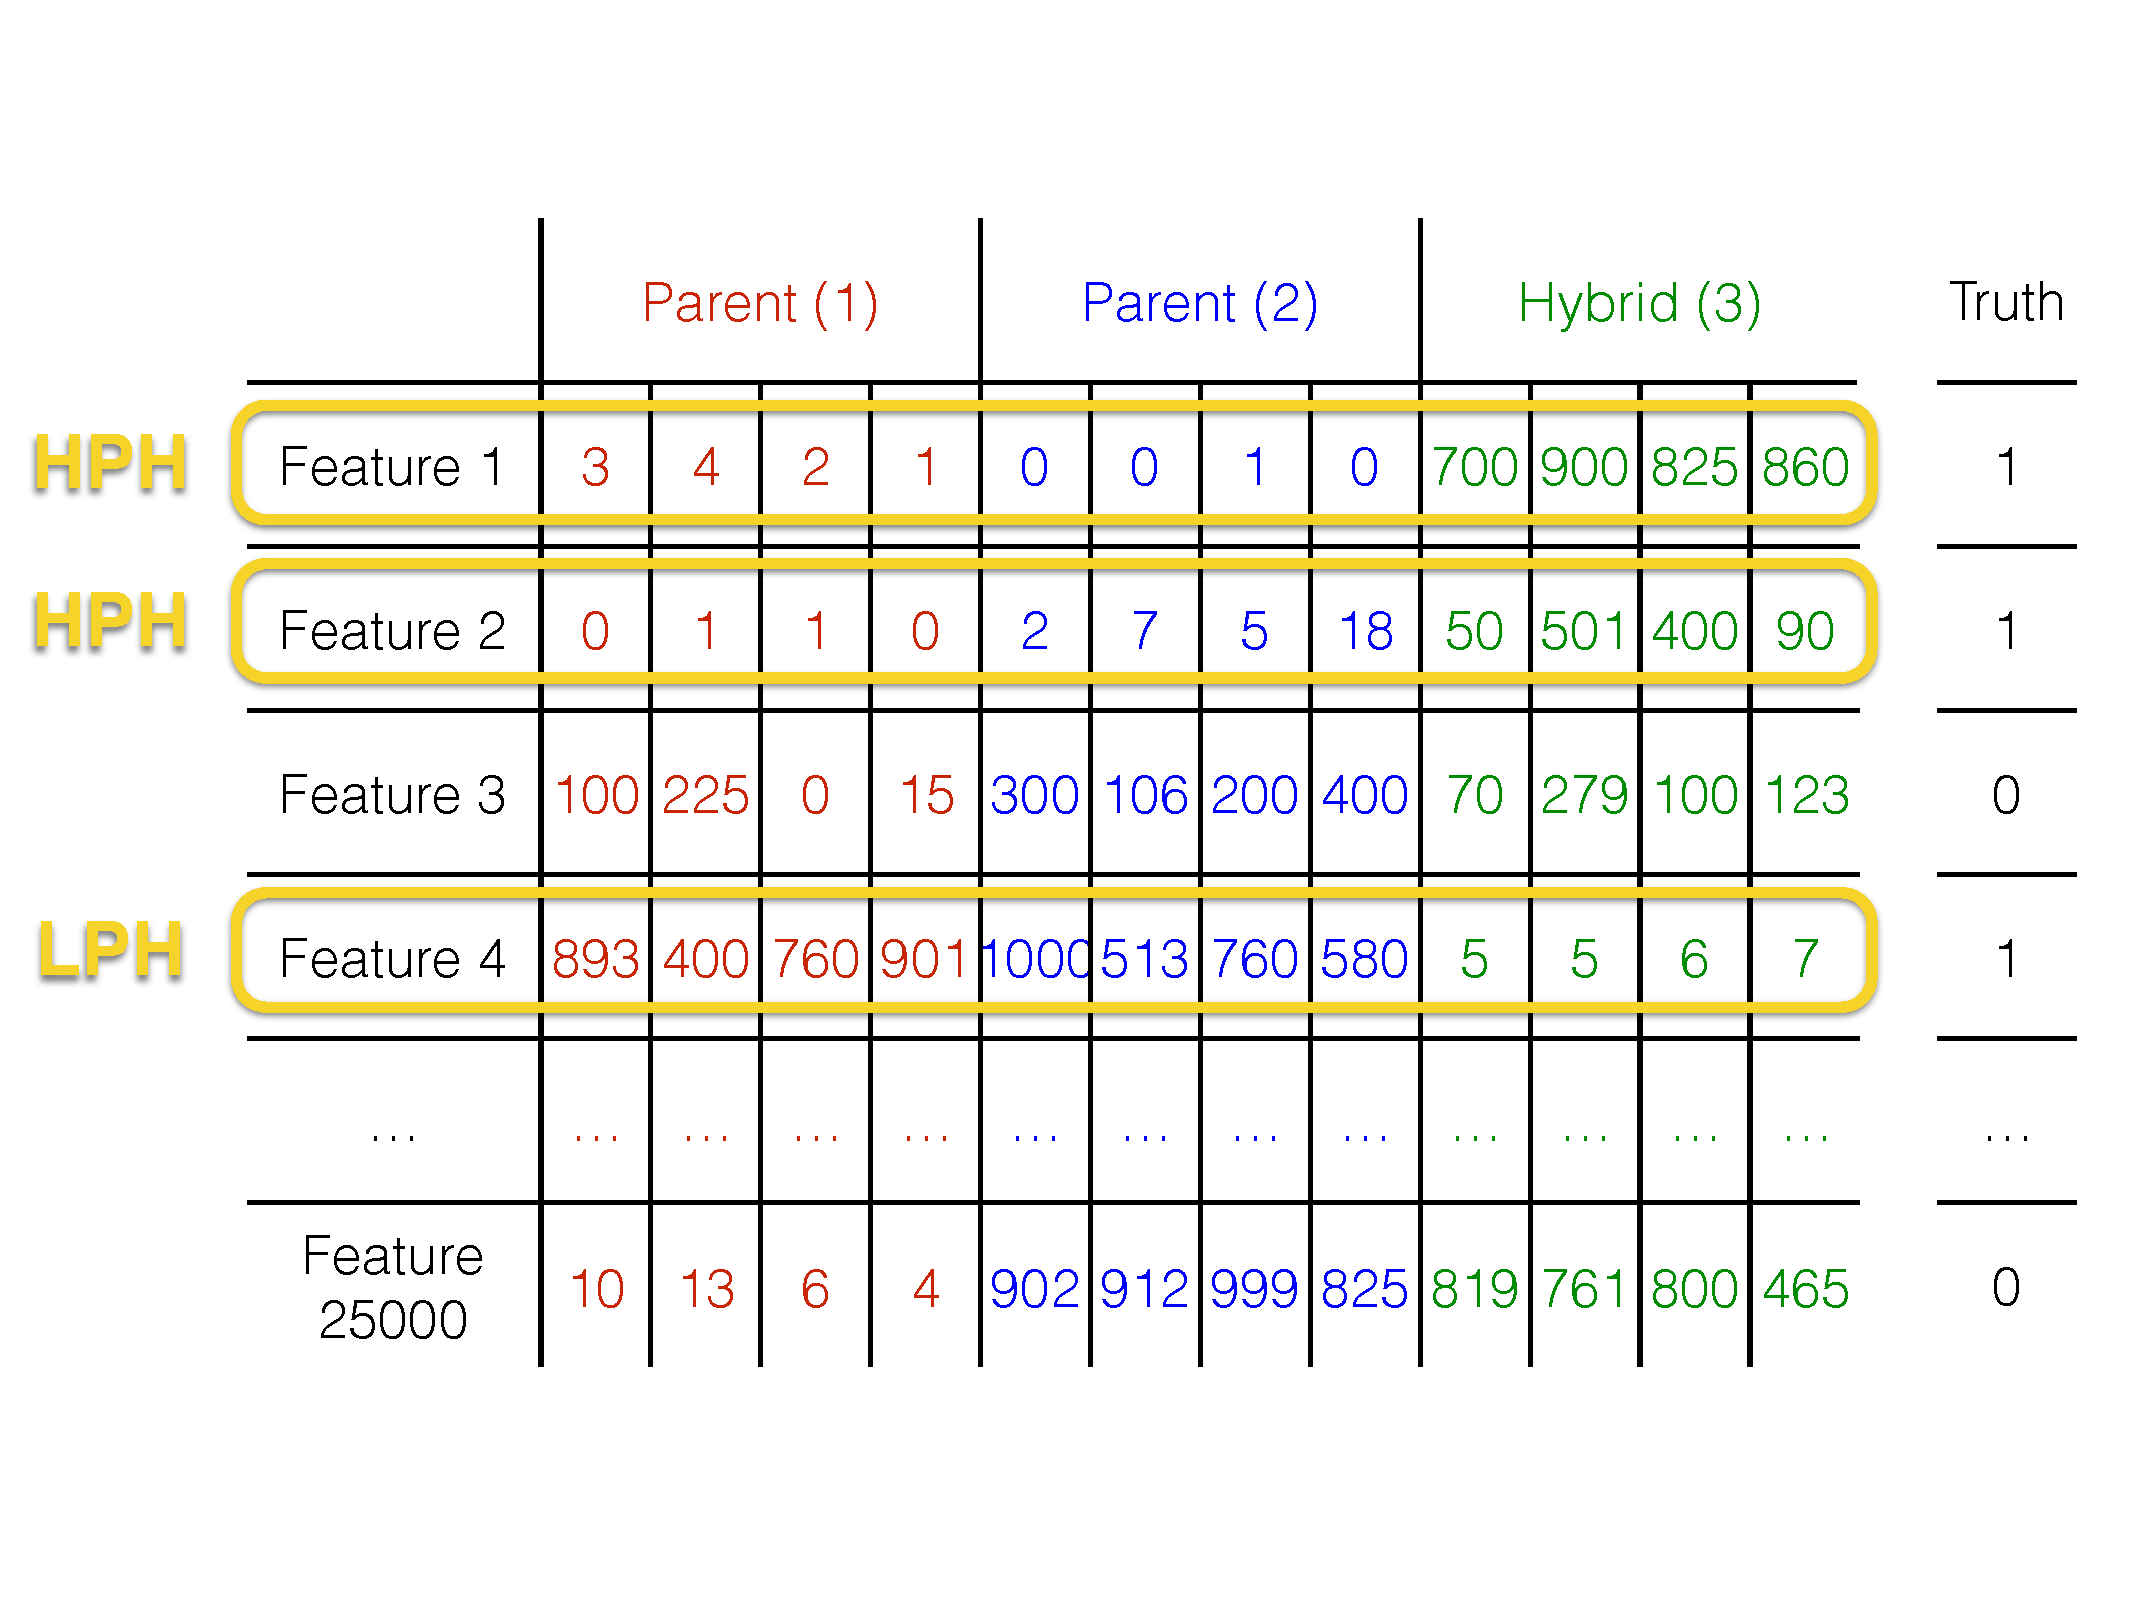
\includegraphics[scale=.28]{data}
\end{center}
\end{frame}

\section{The workflow}

\begin{frame}
\frametitle{Simulation workflow}

\begin{itemize}
\item Simulate 30 datasets:
\begin{itemize}
\item 10 datasets with 4 samples (libraries, columns, etc.) per group
\item 10 with 8 per group
\item 10 with 16 per group
\end{itemize}
\pause \item For each simulated dataset, test for heterosis with
\begin{itemize}
\item empirical Bayes with STAN (Eric's method)
\item {\tt edgeR} 
\item {\tt baySeq}
\item {\tt ShrinkBayes}
\end{itemize}
\pause \item Compare methods with ROC curves
\end{itemize}
\end{frame}

\section{Simulated data}


\begin{frame}
\frametitle{Apply {\tt edgeR} to real data to get simulation parameters}
\begin{center}
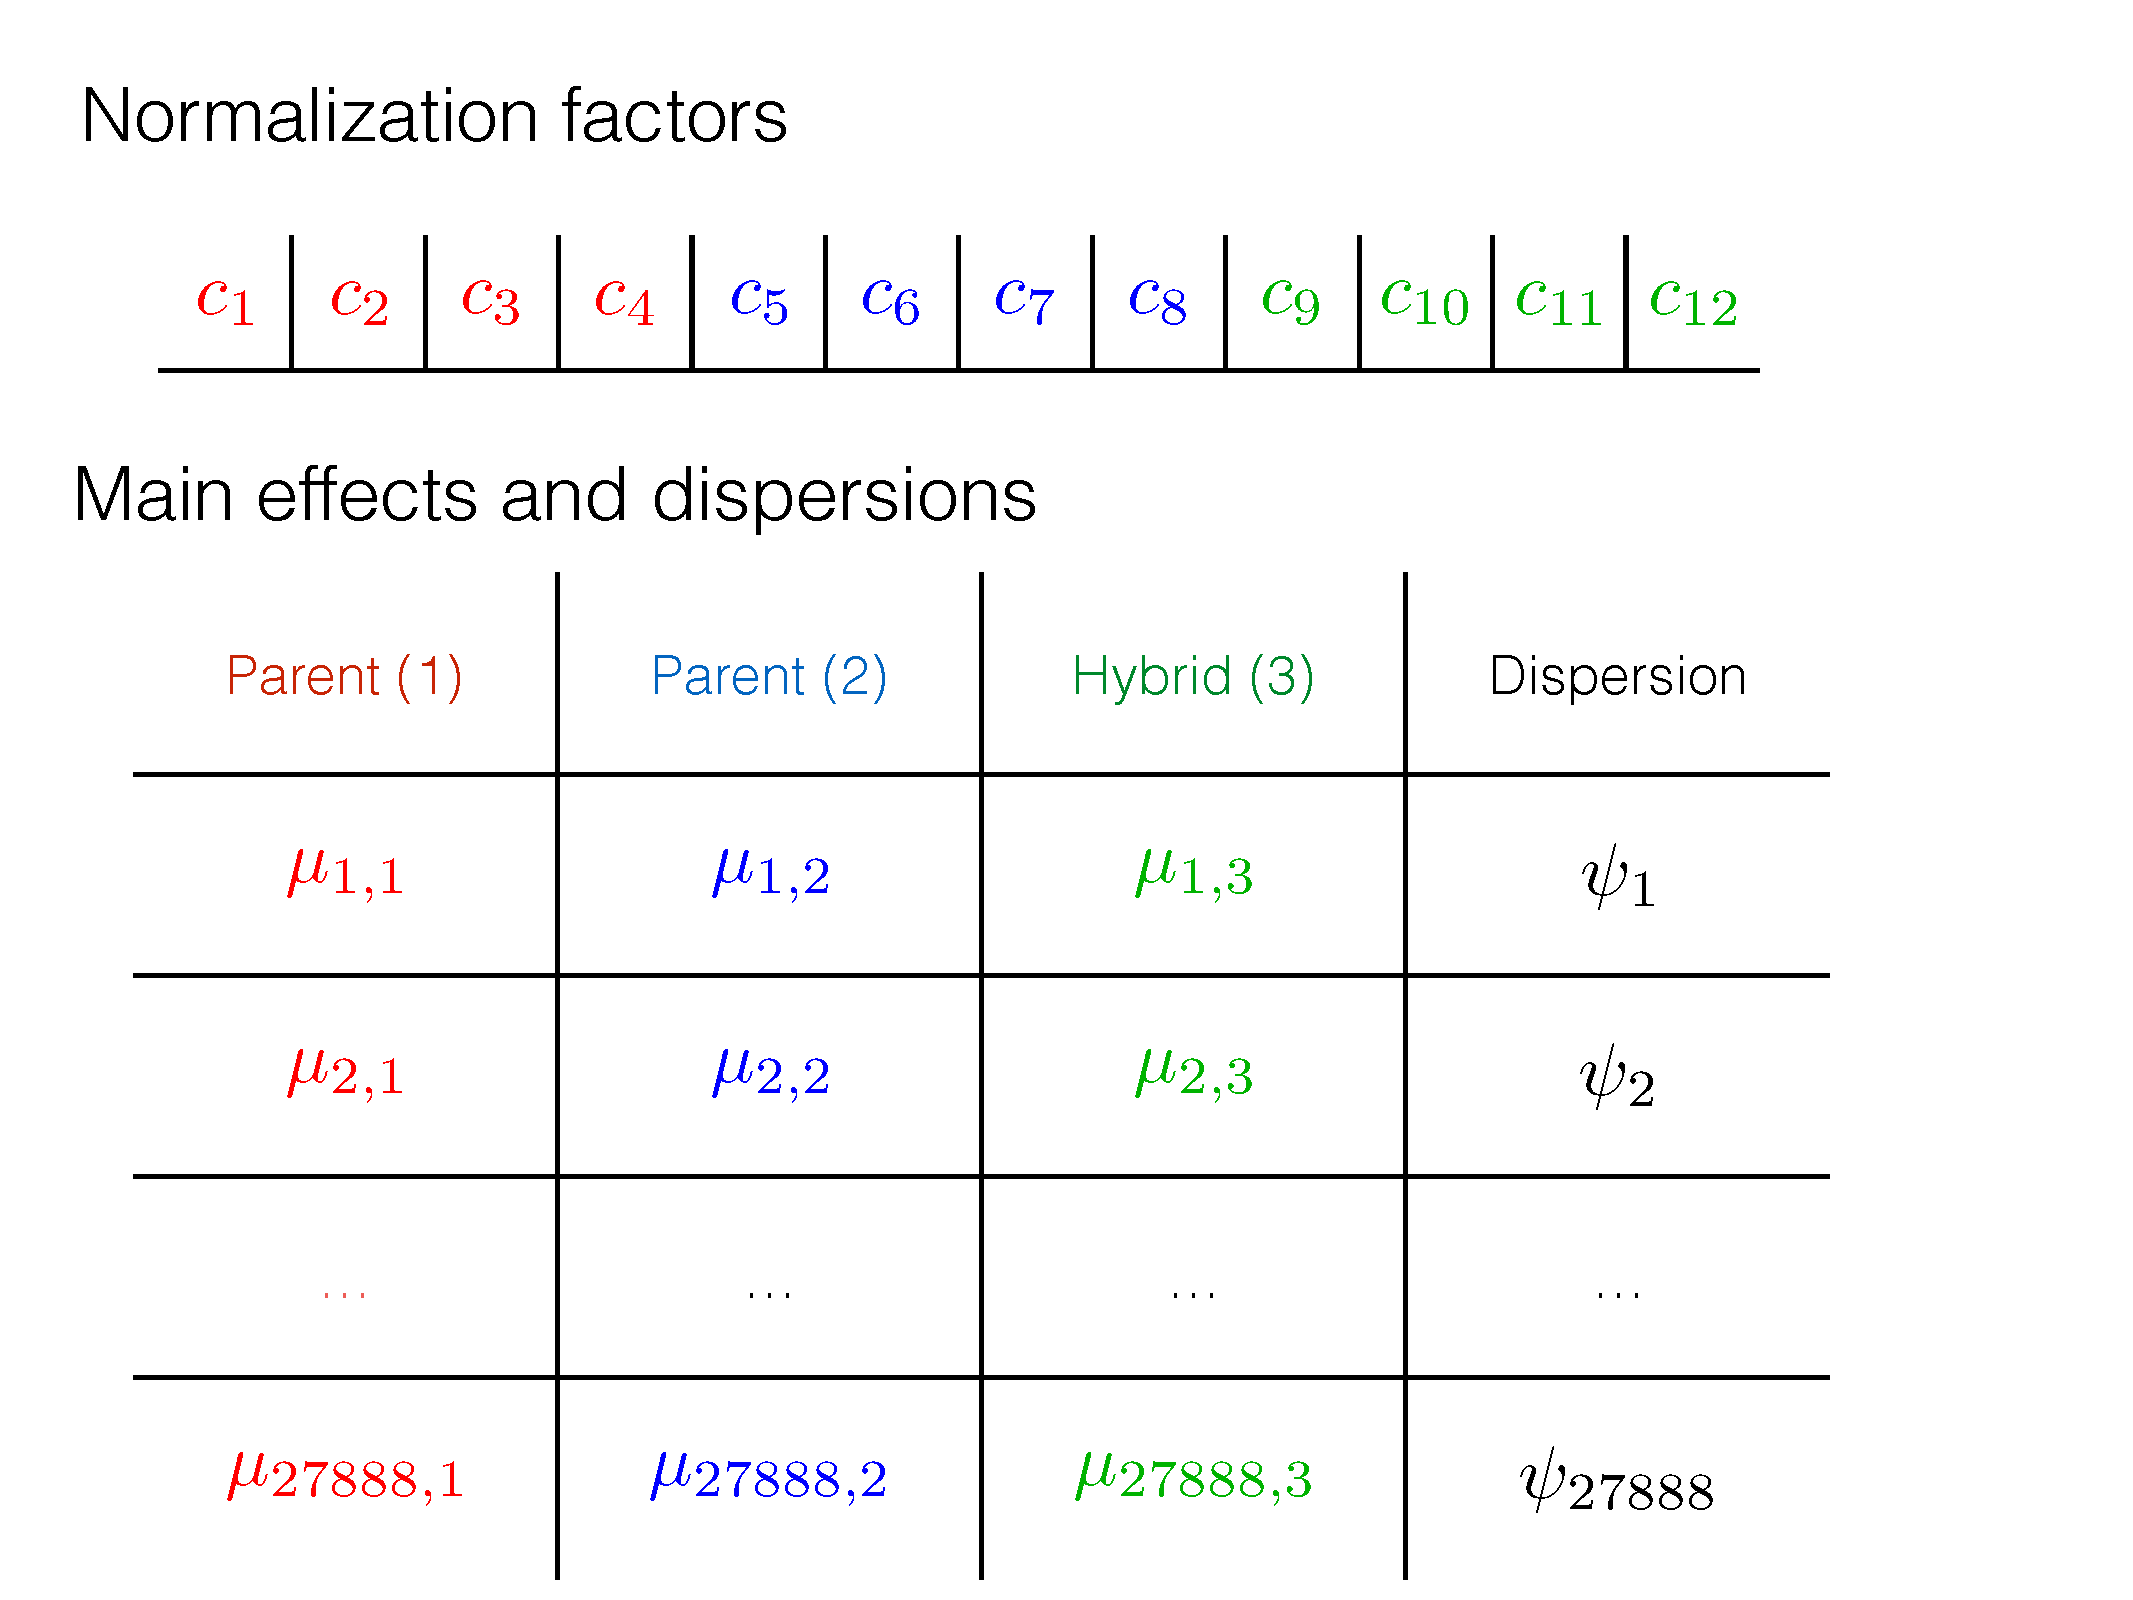
\includegraphics[scale=.25]{parms}
\end{center}
\end{frame}




\begin{frame}
\frametitle{Generating the data}

\begin{itemize}
\item Does feature $f$ truly have heterosis?
\begin{align*}
\text{truth}_f = I(&{\color{dkgreen}\mu_{f, 3}} > \max({\color{red}\mu_{f, 1}}, {\color{blue}\mu_{f, 2}}) \text{ or } \\ &{\color{dkgreen}\mu_{f, 3}} < \min({\color{red}\mu_{f, 1}}, {\color{blue}\mu_{f, 2}}))
\end{align*}

\pause 

\item For a dataset with 4 libraries per group,


\begin{align*}
y_{f, i} &\mathop{\sim}^{\text{iid}} NB\left (\exp \left ( c_{i} + \mu_{f, t(i)} \right ), \ \psi_f  \right )
\end{align*}

\begin{itemize}
\item $t(i)$ is the group of library $i$.
\pause \item Resimulate to increase the number of libraries per group.
\end{itemize}



\pause \item Remove extremely low-count features.
\pause \item Take a random subset of 25000 features from the remaining ones.
\end{itemize}
\end{frame}

\begin{frame}
\frametitle{Mock example data with 4 samples per treatment group}
\begin{center}
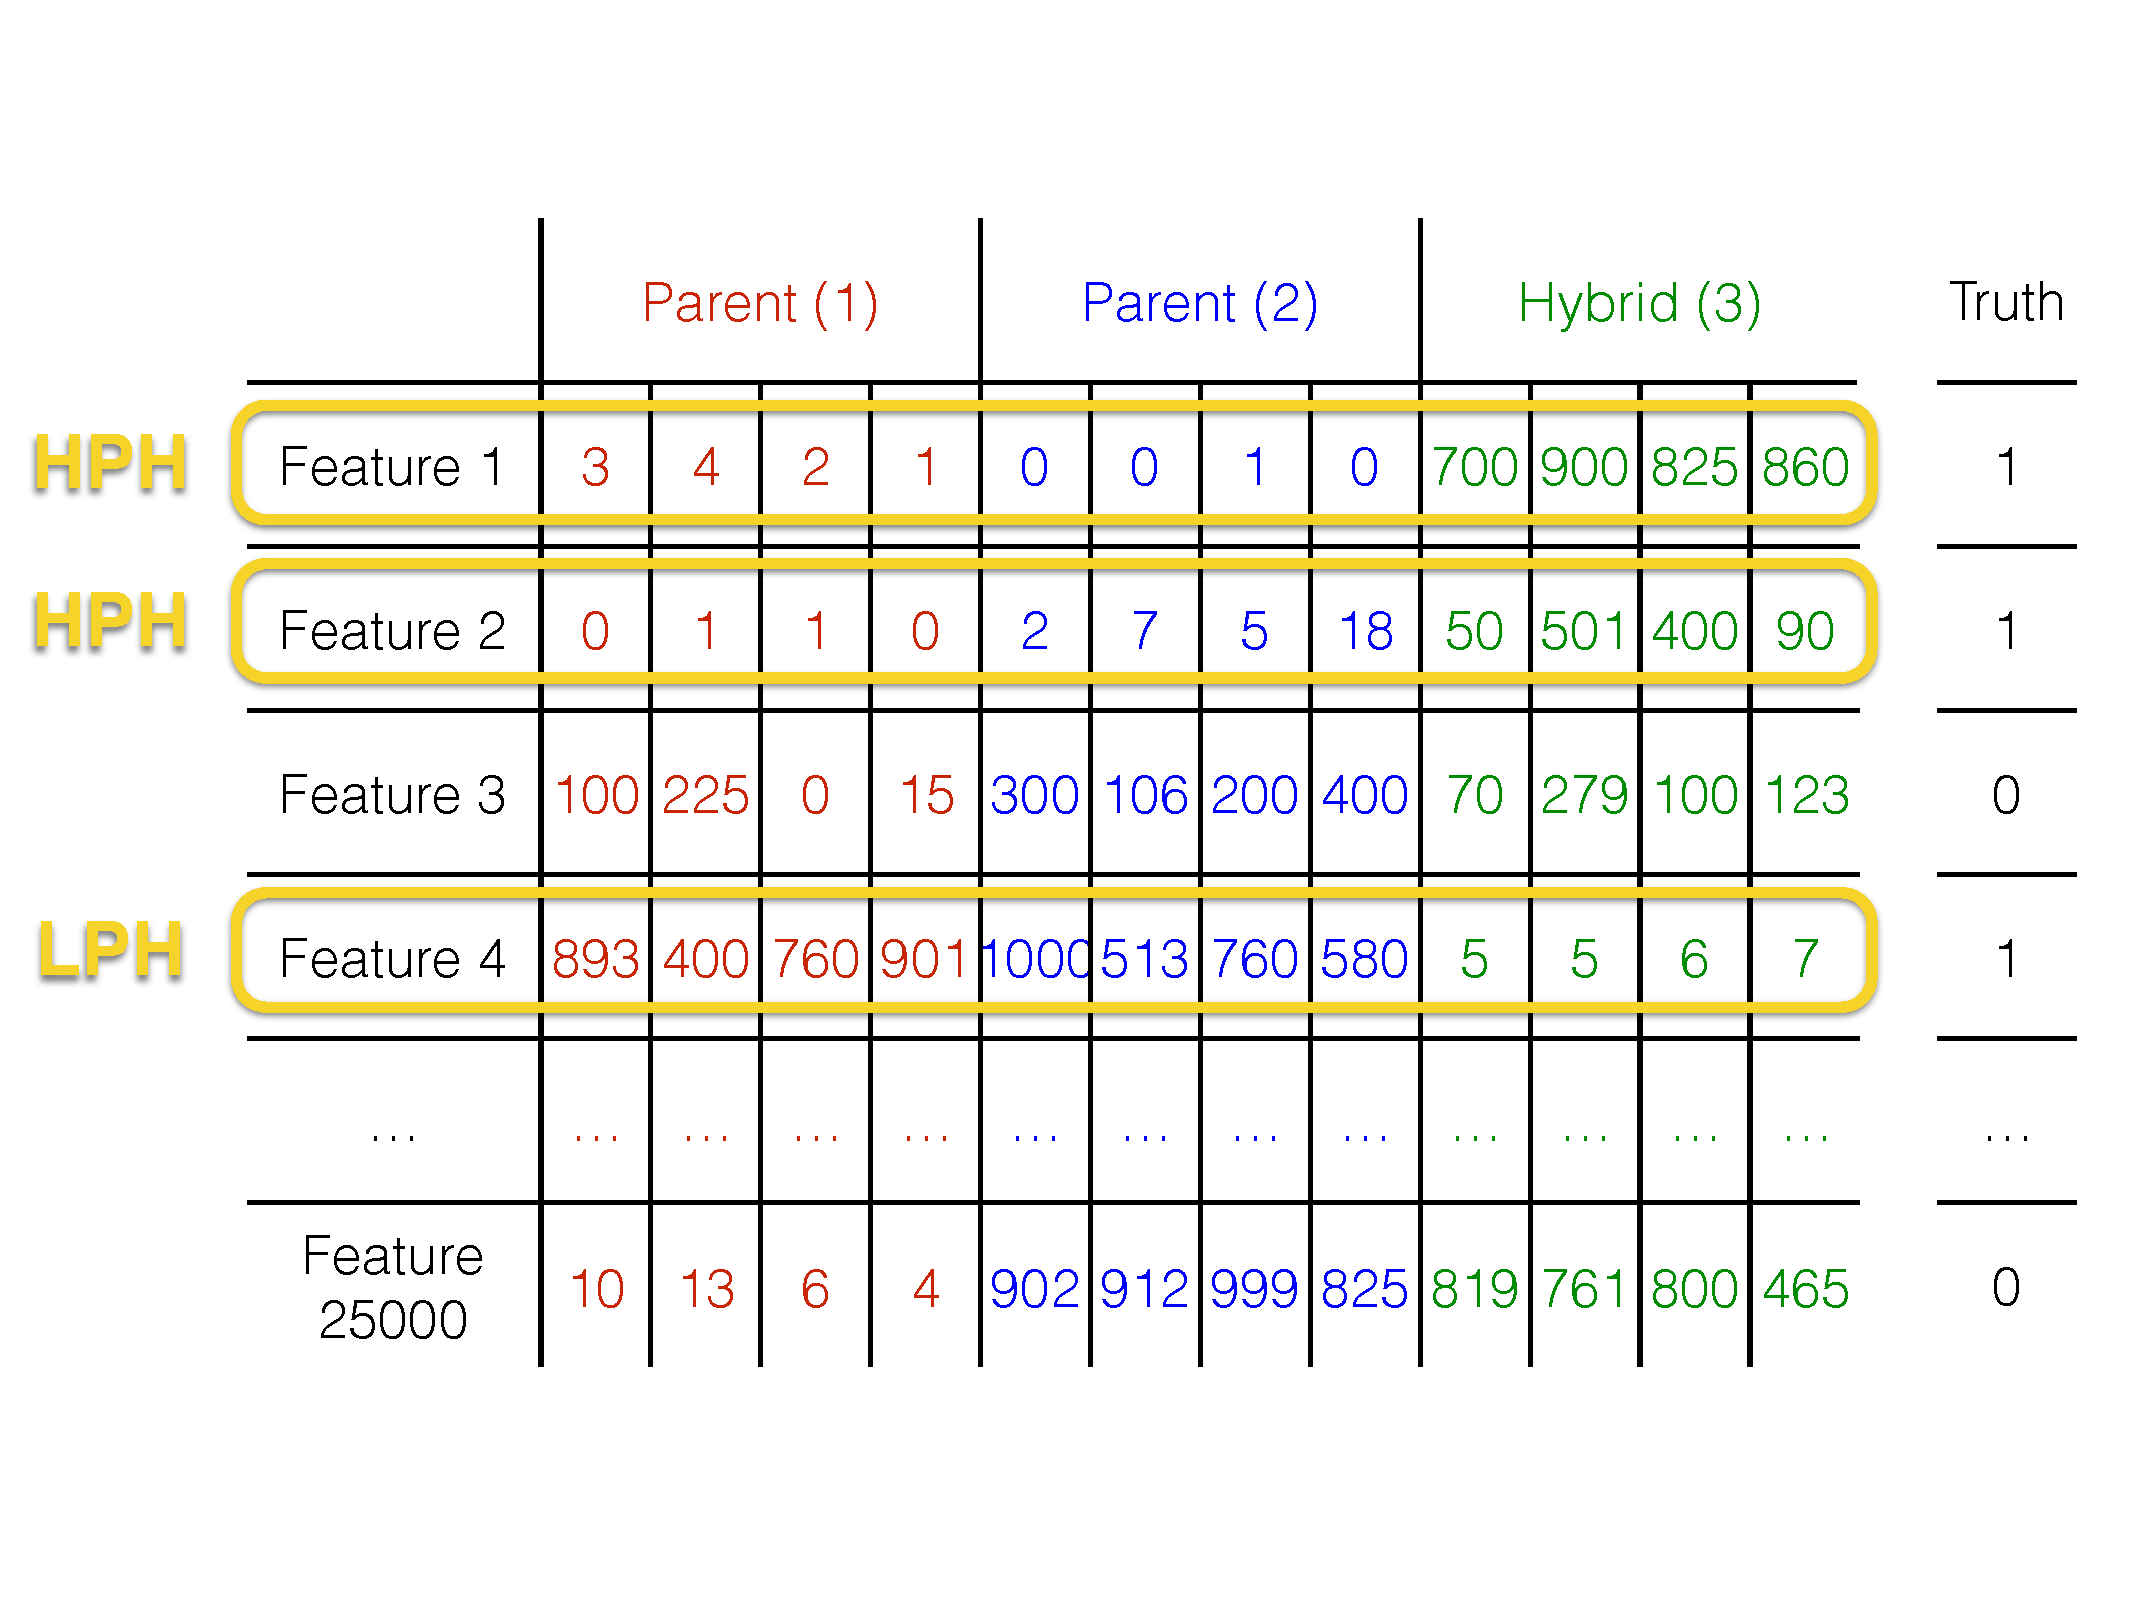
\includegraphics[scale=.28]{data}
\end{center}
\end{frame}

\section{The contenders}

\subsection{{\tt edgeR}}

\begin{frame}
\frametitle{{\tt edgeR}}

\begin{itemize}
\item Fit a loglinear model to estimate main effects $\mu_{f, t}$
\begin{itemize}
\item Feature $f = 1, \ldots, 25000$
\item Treatment group $t = $ {\color{red} 1 (parent)}, {\color{blue} 2 (parent)}, {\color{dkgreen} 3 (hybrid)}
\end{itemize}
\pause \item Likelihood ratio tests to get p-values ${\color{red} p_{f, 1}}, \ {\color{blue} p_{f, 2}}$

\begin{align*}
H_{0, 1}:{\color{dkgreen} \mu_{f, 3}} &= {\color{red}\mu_{f, 1}} \qquad H_{a, 1}: {\color{dkgreen}\mu_{f, 3}} \ne {\color{red} \mu_{f, 1}} \\
H_{0, 2}: {\color{dkgreen} \mu_{f, 3}} &= {\color{blue} \mu_{f, 2}} \qquad H_{a, 2}: {\color{dkgreen}\mu_{f, 3}} \ne {\color{blue}\mu_{f, 2}}
\end{align*}


\pause \item Final p-value:

\end{itemize}


\begin{align*}
p_{f, \text{{\tt edgeR}}} &= \begin{cases}
{\color{red}p_{f, 1}}/{2} &{\color{dkgreen} \wh{\mu}_{f, 3} }< {\color{red}\wh{\mu}_{f, 1}} \le {\color{blue}\wh{\mu}_{f, 2}} \text{ or }{\color{dkgreen}\wh{\mu}_{f, 3}} > {\color{red}\wh{\mu}_{f, 1}} \ge {\color{blue}\wh{\mu}_{f, 2}} \\
{\color{blue}p_{f, 2}}/{2} &{\color{dkgreen} \wh{\mu}_{f, 3}} < {\color{blue}\wh{\mu}_{f, 2}} \le {\color{red}\wh{\mu}_{f, 1}} \text{ or }{\color{dkgreen}\wh{\mu}_{f, 3}} > {\color{blue}\wh{\mu}_{f, 2}} \ge {\color{red}\wh{\mu}_{f, 1}} \\
1 & {\color{red}\wh{\mu}_{f, 1}} \le {\color{dkgreen} \wh{\mu}_{f, 3}} \le {\color{blue}\wh{\mu}_{f, 2}} \text{ or } {\color{blue}\wh{\mu}_{f, 2}} \le{\color{dkgreen} \wh{\mu}_{f, 3}} \le {\color{red}\wh{\mu}_{f, 1}}
\end{cases}
\end{align*}
\end{frame}

\subsection{{\tt ShrinkBayes}}

\begin{frame}
\frametitle{{\tt ShrinkBayes}}
\begin{itemize}
\item Built on {\tt inla} (integrated nested Laplace approximation).
\pause \item empirical Bayes with a zero-inflated NB likelihood and normal priors.
\pause \item I reparameterize

\begin{align*}
\phi_f &= \frac{{\color{red}\mu_{f, 1}} + {\color{blue}\mu_{f, 2}}}{2} \qquad \text{(parental mean)} \\
\alpha_f &= \frac{{\color{blue}\mu_{f, 2}} - {\color{red}\mu_{f, 1}}}{2} \qquad \text{(half parental difference)} \\
\delta_f &= {\color{dkgreen}\mu_{f, 3}} - \frac{{\color{red}\mu_{f, 1}} + {\color{blue}\mu_{f, 2}}}{2} \qquad \text{(hybrid effect)} 
\end{align*}
\end{itemize}
\end{frame}

\begin{frame}
\frametitle{{\tt ShrinkBayes}}

\begin{align*}
\alpha_f &= \text{ half parental difference} \\
\delta_f &= \text{ hybrid effect}
\end{align*}

\begin{itemize}
\item Use contrasts to calculate final posterior probabilities of heterosis:

\end{itemize}


\begin{align*}
p_{f, \text{\tt ShrinkBayes}} &= \begin{cases}
0 & \left |\wh{\delta}_f  \right | < \left | \wh{\alpha}_f  \right | \text{, o.w.:} \\
P(\delta_f + \alpha_f > 0 \mid \text{data}) & \wh{\delta}_f > -\wh{\alpha}_f \\
P(\delta_f - \alpha_f > 0 \mid \text{data}) & \wh{\delta}_f > \wh{\alpha}_f \\
P(\delta_f - \alpha_f < 0 \mid \text{data}) & \wh{\delta}_f < \wh{\alpha}_f \\
P(\delta_f + \alpha_f < 0 \mid \text{data}) & \wh{\delta}_f < -\wh{\alpha}_f
\end{cases}
\end{align*}
\end{frame}


\subsection{{\tt baySeq}}

\begin{frame}
\frametitle{{\tt baySeq}}
\begin{itemize}
\item Estimate main effects $\mu_{f, t}$ using {\tt edgeR}.
\pause \item Calculate the posterior probability that each feature satisfies:

\begin{center}
\begin{tabular}{l|l}
Model & Constraint \\ \hline
$M_1$ & All $\mu_{f, t}$'s equal \\
$M_2$ &  ${\color{red}\mu_{f, 1}} = {\color{blue}\mu_{f, 2}}$ \\
$M_3$ & ${\color{red}\mu_{f, 1}} = {\color{dkgreen}\mu_{f, 3}}$ \\
$M_4$ & ${\color{blue}\mu_{f, 2}} = {\color{dkgreen}\mu_{f, 3}}$ \\
$M_5$ &  All $\mu_{f, t}$'s distinct
\end{tabular}
\end{center}

\pause \item Final posterior probabilities of heterosis:

\end{itemize}

\begin{align*}
p_{f, \text{{\tt baySeq}}} &= \begin{cases}
0 & {\color{red}\wh{\mu}_{f, 1}} \le {\color{dkgreen}\wh{\mu}_{f, 3}} \le {\color{blue}\wh{\mu}_{f, 2}}$ or $ \\
& {\color{blue}\wh{\mu}_{f, 2}} \le {\color{dkgreen}\wh{\mu}_{f, 3}} \le {\color{red}\wh{\mu}_{f, 1}} \\
P(M_2 \mid \text{data}) \ + \\ P(M_5 \mid \text{data}) & \text{otherwise}
\end{cases}
\end{align*}

\end{frame}

\section{The contest}

\subsection{ROC (receiver operating characteristic) curves}

\begin{frame}
\frametitle{Calculating false positive rate (FPR) and true positive rate (TPR)}

\begin{itemize}
\item $N_{\text{true}}$ heterosis features, $N_{\text{false}}$ null features.
\pause \item Results of testing each feature for heterosis (25000 columns here):
\end{itemize}

\begin{tabular}{l|l|l|l|l|l|l|l}
rank & 0.802 & 0.935 & 0.539 & 0.001 & $\cdots$ & 0.500 &  0.603  \\ \hline
truth &  0 & 0 & 1 & 1 & $\cdots$ & 1 & 0 
\end{tabular}

\begin{itemize}

\pause \item Sort table by p-value (or other binary classifier)
\end{itemize}

\begin{tabular}{l|l|l|l|l|l|l|l}
rank & 0.000 & 0.001 & 0.005 & 0.006 & $\cdots$ & 0.901 & 1.000  \\ \hline
truth &  1 & 1 & 0 & 1 & $\cdots$ & 0 & 0
\end{tabular}
\end{frame}

\begin{frame}
\frametitle{Calculating false positive rate (FPR) and true positive rate (TPR)}

\begin{itemize}
\pause \item In practice, we would declare the lowest-p-value features to have heterosis.
\end{itemize}

\pause \begin{tabular}{l|l|l|l|l|l|l|l}
rank & {\color{blue} 0.000} & {\color{blue}0.001} & {\color{blue}0.005} & 0.006 & $\cdots$ & 0.901 & 1.000  \\ \hline
truth & {\color{blue}1} & {\color{blue}1} & {\color{blue}0} & 1 & $\cdots$ & 0 & 0
\end{tabular}

\begin{itemize}
\pause \item With 2 heterosis genes and 1 null gene,

\begin{align*}
FPR = \frac{1}{N_{false}} \qquad TPR = \frac{2}{N_{true}}
\end{align*}

\pause \item Repeat for multiple cutoffs to get multiple (FPR, TPR) pairs.
\end{itemize}
\end{frame}


\begin{frame}
\frametitle{Example ROC curves}
\begin{center}
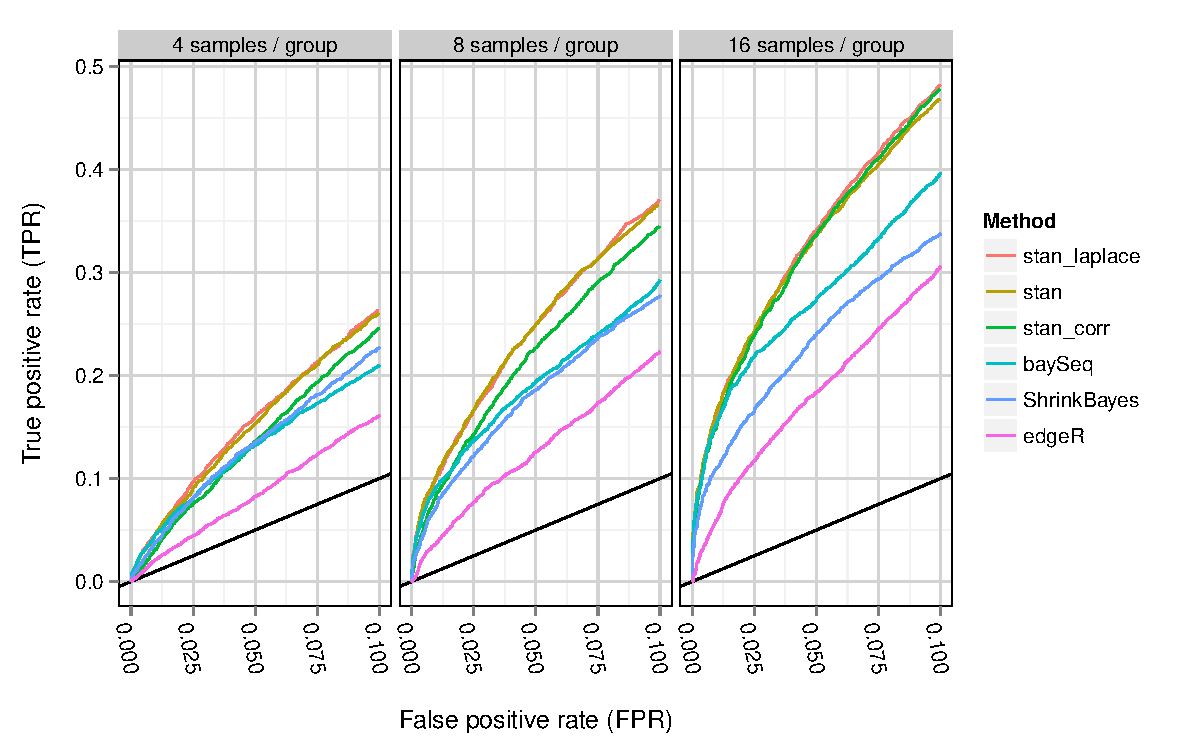
\includegraphics[scale=0.5]{roc}
\end{center}
\end{frame}



\subsection{The results}

\begin{frame}
\frametitle{Areas under ROC curves}
\begin{center}
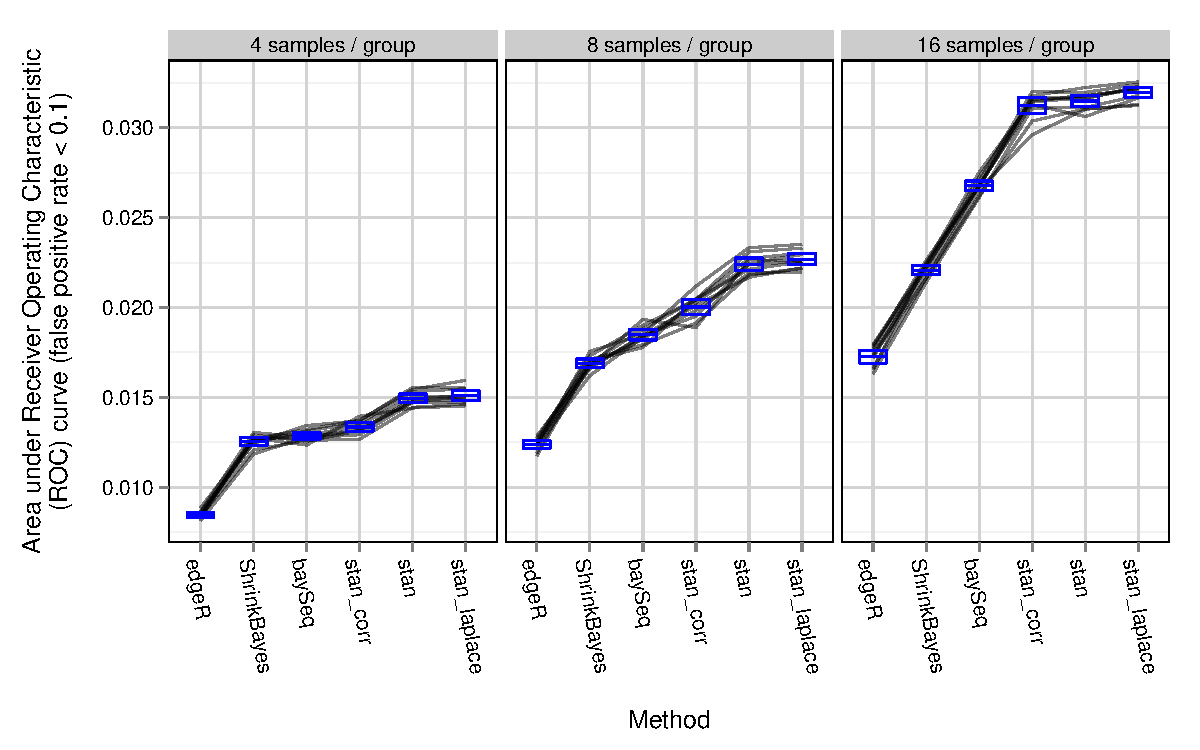
\includegraphics[scale=0.5]{auc1}
\end{center}
\end{frame}

\begin{frame}
\frametitle{Areas under ROC curves}
\begin{center}
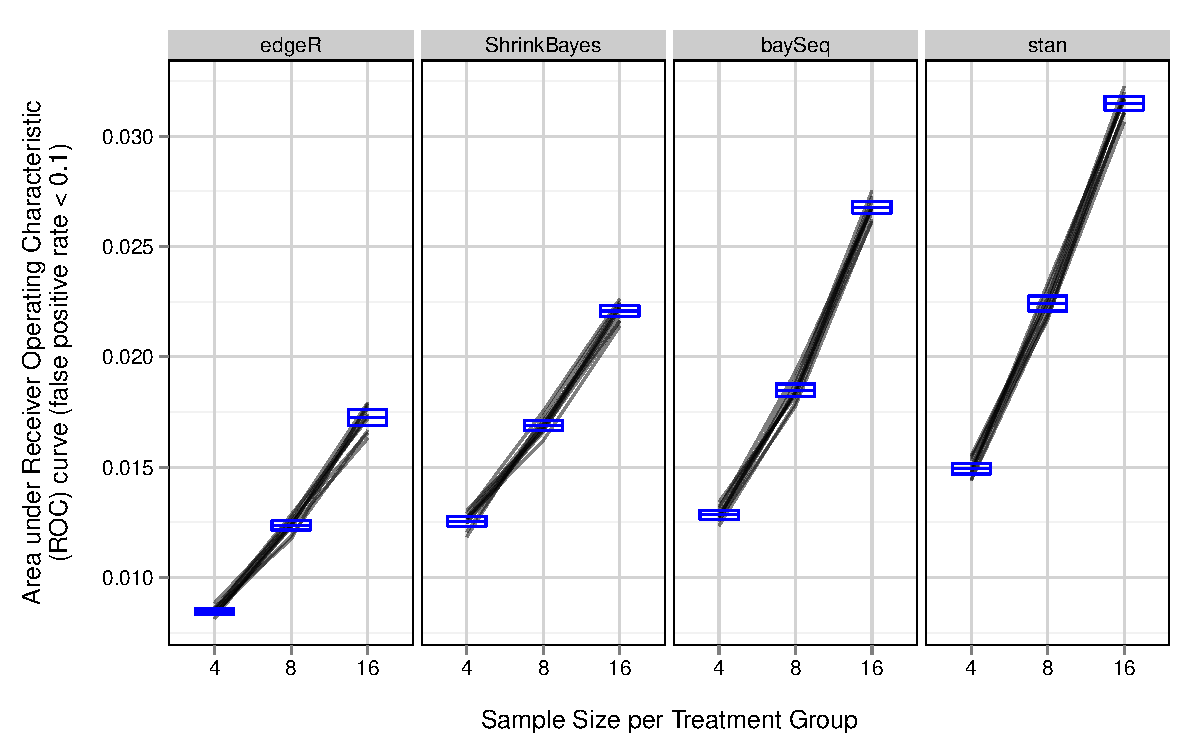
\includegraphics[scale=0.5]{auc2}
\end{center}
\end{frame}

\end{document}